\documentclass{article}
\usepackage{graphicx}
\usepackage{amsmath} % For better math support
\usepackage{amssymb}
\usepackage[a4paper, margin=.2in]{geometry} % Adjust margins as needed
\usepackage{tikz} % For drawing
% Define the page border

\begin{document}

    Current of capacitor equals current of supply:
    
    \[
    I_{C} = I_F
    \]
    
    \[
    C \frac{dV_c}{dt} = \frac{0-V_{out}}{R_f}   
    \]
    
    \[
    V_{out} = C.R_f\frac{dV_c}{dt}
    \]
    
    \[
    \because V_{in} = V_C
    \]
    
    \[
    \therefore V_{out} = C.R_f\frac{dV_{in}}{dt}
    \]
    
    \text{let's look at \({V_{out}}\) in terms of impedance}
    \[
    V_{out}=\frac{-R_f}{X_C}.V_{in} = -2.\pi .R_f.C.F.V_{in}
    \]
    
    from pervious equation, At high frequencies the op amp will act as open loop gain
    \begin{figure}[h]
        \centering
        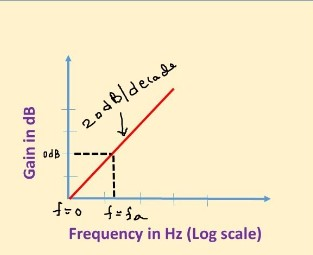
\includegraphics[width=0.4\textwidth]{ideal.jpg}
    \end{figure}
    
    \[
    F_a=\frac{1}{2\pi R_f.C}
    \]
    
    the increase of gain towards \(\infty\) not gonna happen because the open loop gain will limit it
    \begin{figure}[h]
        \centering
        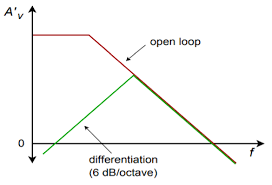
\includegraphics[width=0.3\textwidth]{practical.png}
    \end{figure}

some limitations of ideal Op-amp as differentiatior
\[
\mathcal{A} \ \text{. Input impedance } Z_{in} = X_c
\]
\text{So at low frequencies, the input impedance is small.}
\\
\text{To overcome this problem, we have to insert a resistance in series with the capacitor.}

\begin{figure}[h]
    \centering
    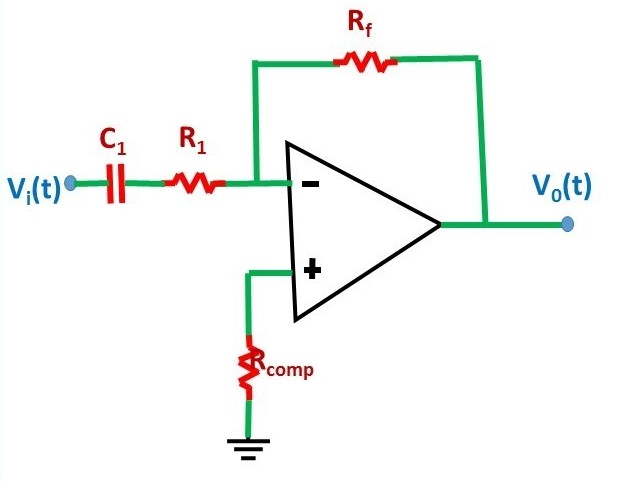
\includegraphics[width=0.2\textwidth]{practical2.jpg}    
\end{figure}
\[
Z_{in}=\sqrt{X_C^2 + R_1^2}
\]

\[
\mathcal{B} \ \text{. increse stabilty at high frequencies }
\]

\text{to do that we gonna introduce capacitor in parallel with \(R_F\)}
\begin{figure}[h]
    \centering
    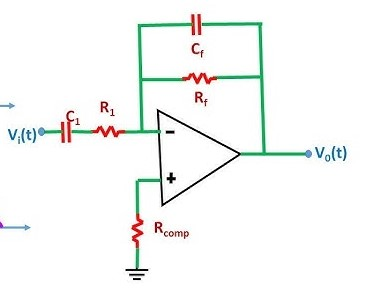
\includegraphics[width=.3\textwidth]{practical3.jpg}    
\end{figure}

\text{we have two Cut off frequencies one for differentiatior and the other of integrator}
\begin{figure}[h]
    \centering
    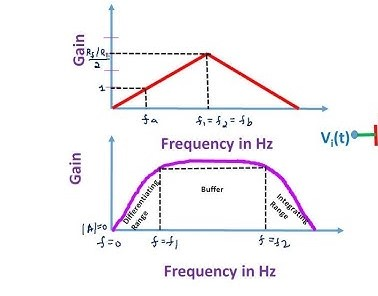
\includegraphics[width=.3\textwidth]{practical4.jpg}
\end{figure}

\[
F_1 =\frac{1}{2\pi.R_1.C_1} \qquad
F_2 =\frac{1}{2\pi.R_f.C_f}
\]
\end{document}